\chapter{Workflow (as is) na notação BPMN}\label{sec:4}

O objetivo do workflow AS-IS é representar a situação atual de um processo organizacional, o mapeando e documentando para melhor compreensão do processo como um todo. A Figura~\ref{fig:workflow-as-is} apresenta o fluxo atual de atividades do sistema.

\begin{figure}[htbp]
    \caption{Workflow AS-IS}
    \label{fig:workflow-as-is}
    \centering
    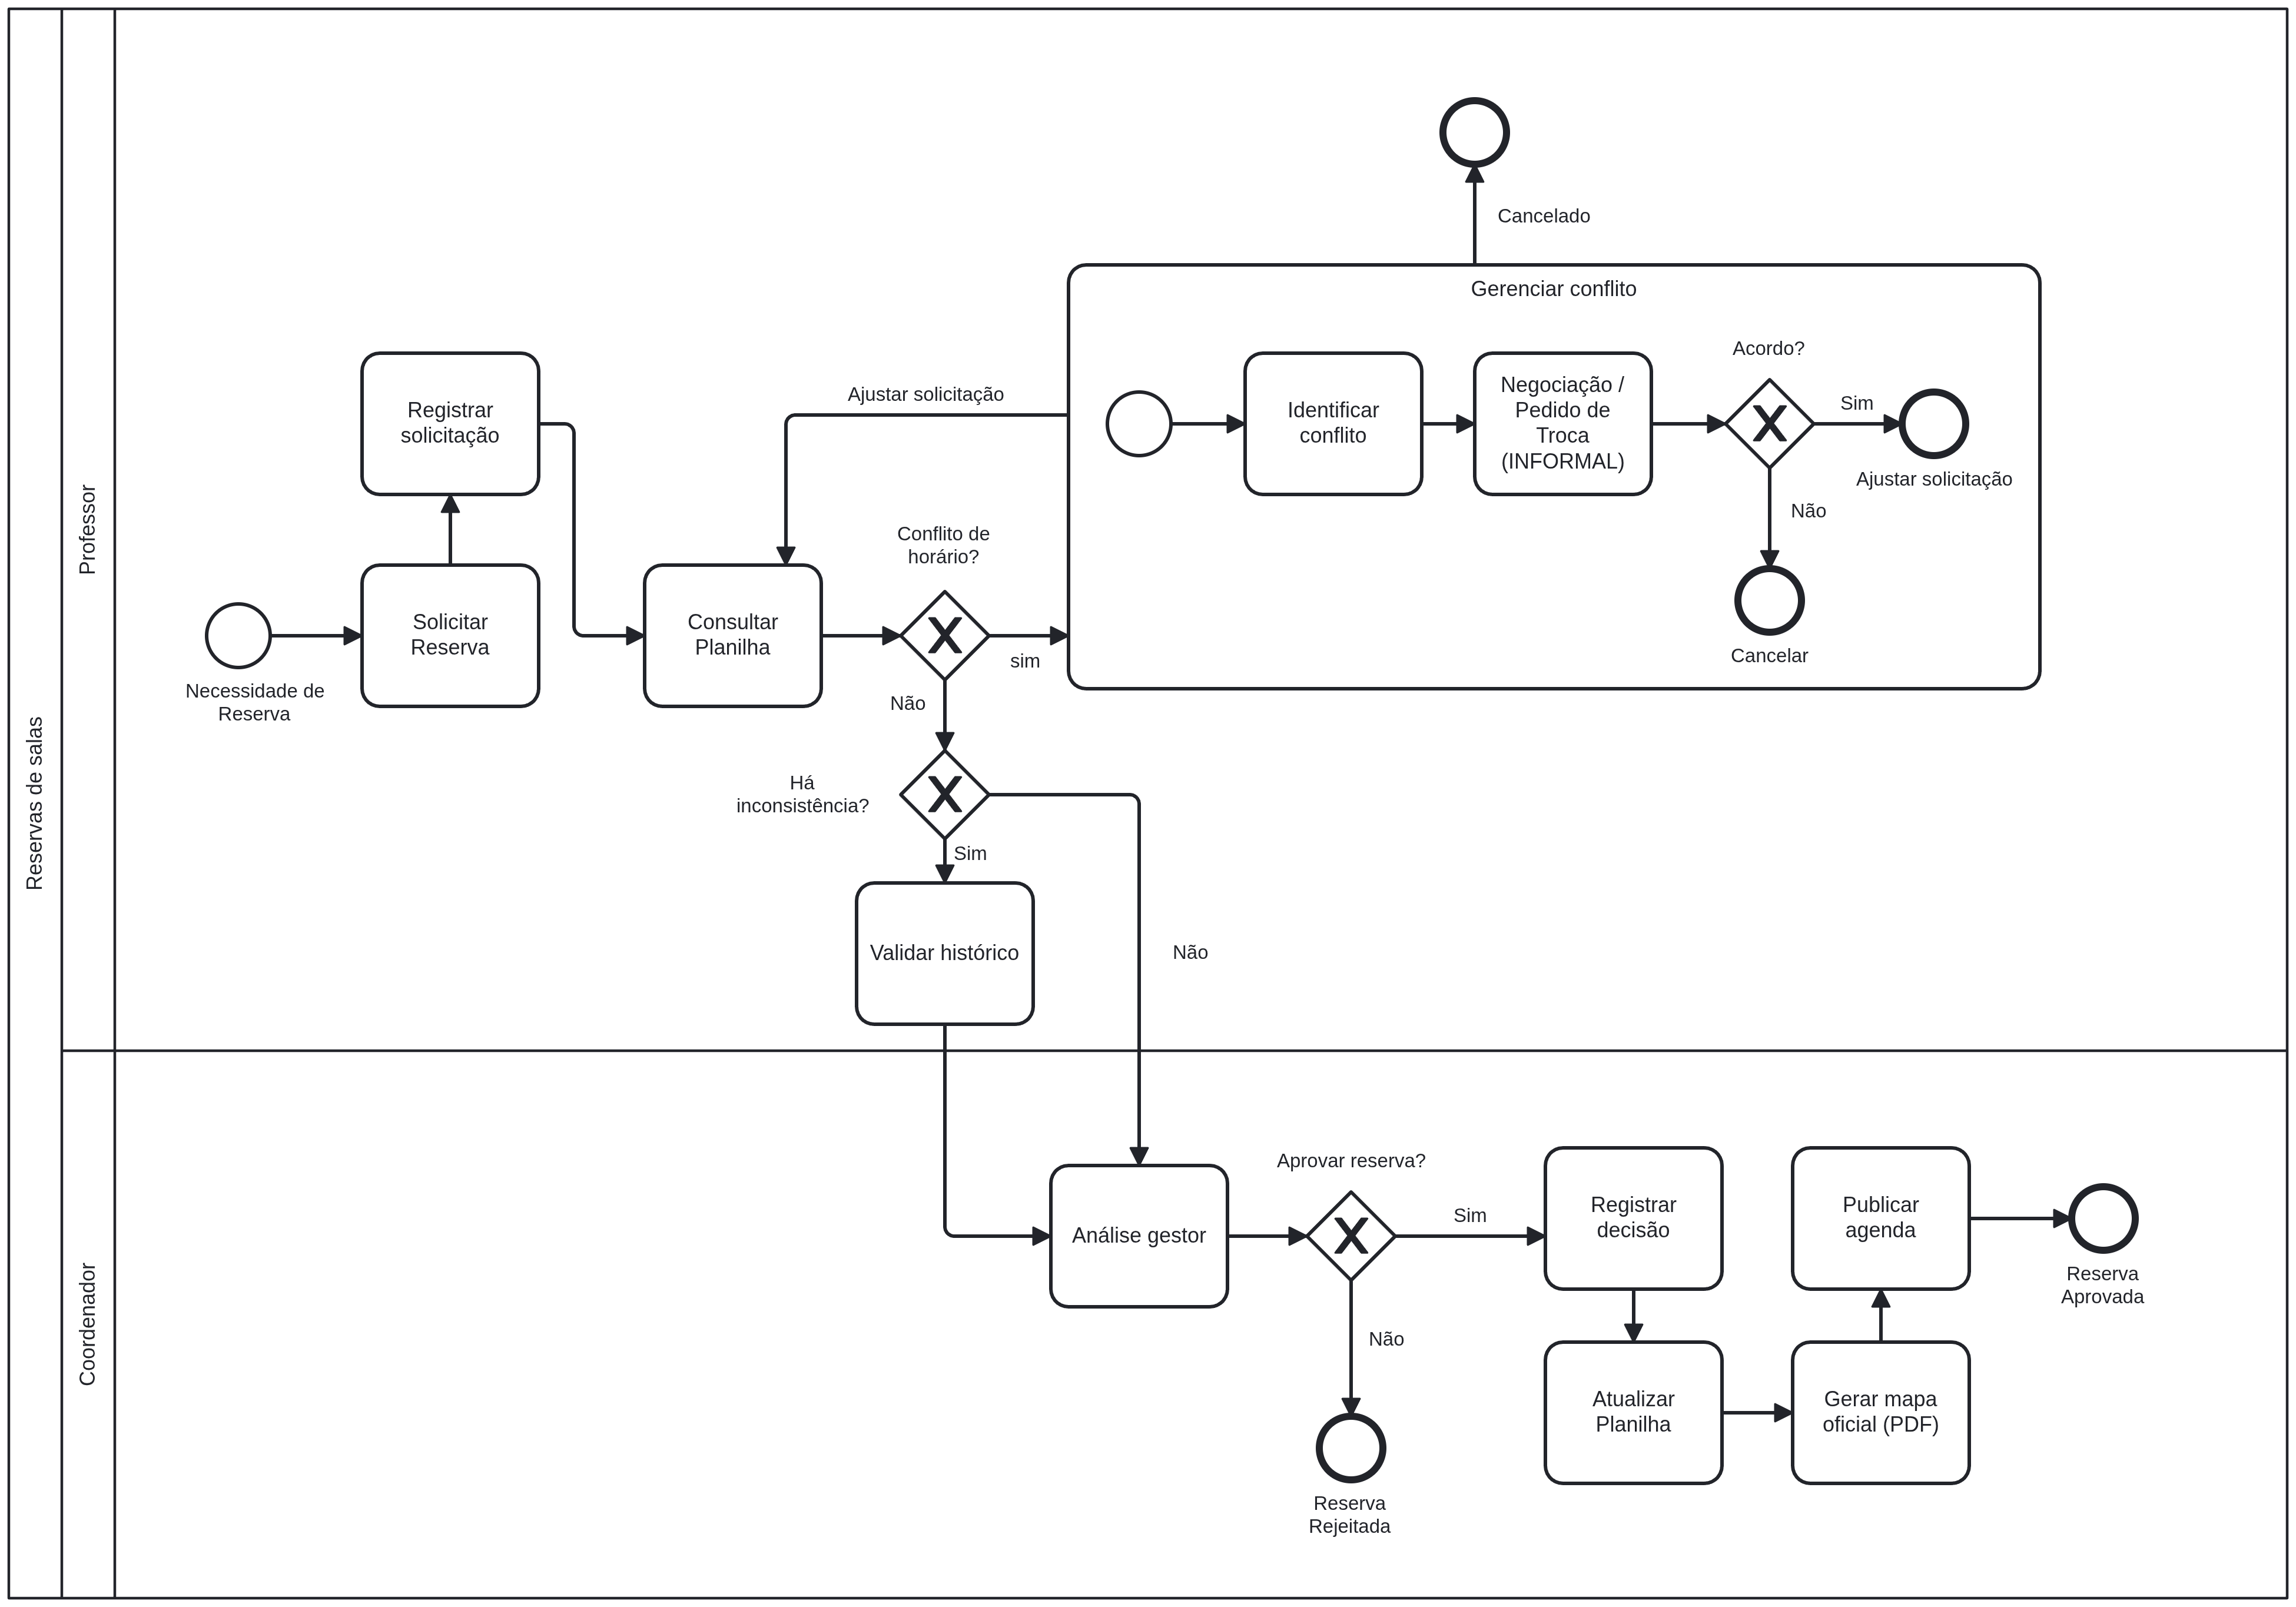
\includegraphics[width=0.8\textwidth]{imagens/workflow-as-is.png}

    {\footnotesize \textbf{Fonte:} O autor.}
\end{figure}